\documentclass[a4paper]{article}

\usepackage{a4wide}
\usepackage{amssymb}
\usepackage{xcolor}
\usepackage{comment}
\usepackage{graphicx}

\title{Elektronisch stemmen}
\author{
Mick van Gelderen \\ 4091566 \and 
Mick de Lange \\ 1534068 \and
Salim Salmi \\ \TODO{stdnr}
}


\newcommand{\TODO}[1]{{\color{red}\textbf{TODO: #1}}}

\usepackage{amsmath}
\begin{document}

\thispagestyle{plain}
\maketitle

\hfill \\ \\ \\ \\ \\ \\ \\ \\ \\ \\
\begin{figure}[htp]
\centering
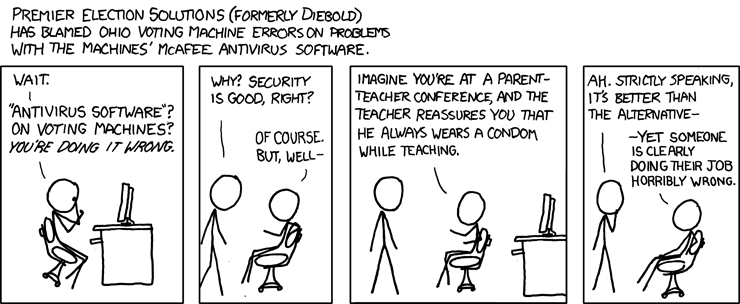
\includegraphics[width=\textwidth]{media/voting_machines.png}
\label{fig:voting-machines}
\begin{comment}
Randall Munroe, (2013), Voting Machines [ONLINE]. Available at: http://imgs.xkcd.com/comics/voting_machines.png [Accessed 15 March 13].
\end{comment}
\end{figure}

\newpage

\thispagestyle{plain}

\section*{Voorwoord}
Dit artikel is geschreven door 3 studenten Technische Informatica aan de Technische Universiteit Delft voor het vak `informatietechnologie en waarden'. Het belicht een ethische kwestie van verschillende standpunten aangesterkt met literatuur uit het vakgebied en de filosofie. 

\newpage

\thispagestyle{plain}
\renewcommand{\contentsname}{Inhoud} 
\tableofcontents

\newpage

\section{Inleiding}

\TODO{Voorstel andere onderzoeksvraag (Naar mijn mening beter): '' Goed normatief :p}

In de afgelopen jaren is er veel te doen geweest rondom elektronisch stemmen. Zo zijn er een aantal proeven geweest, zowel in binnen als buitenland met het invoeren van stemcomputers. Er zijn duidelijke voordelen, zo hoeven er geen biljetten meer met de hand geteld te worden en is de uitslag vrijwel direct beschikbaar. Er zijn echter ook duidelijke ethische en morele problemen met het elektronische stemmen, denk hierbij aan privacy, anonimiteit en veiligheid. Veel mensen hebben er moeite mee dat bij elektronisch stemmen het proces niet meer inzichtelijk is of zijn bang dat de stemmen mogelijk gekoppeld kunnen worden aan de persoon, waar dat met papieren stembiljetten niet mogelijk is.
Er zijn op het gebied van elektronisch stemmen dan ook veel problemen, maar ook voordelen. Wij willen in dit artikel in gaan op deze aspecten en onderzoeken wat deze problemen en voordelen met zich mee brengen en hoe men tot bepaalde beslissingen is gekomen.

\subsection{Onderzoeksvraag}

Onze onderzoeksvraag luidt: ``Zouden we over moeten stappen op elektronisch stemmen?''. Deze vraag geeft zowel de twijfel over de duidelijke voordelen van elektronisch stemmen weer, als de onderliggende redenen om nog altijd gebruik te blijven maken van papieren stembiljetten.

\section{Argumenten voor}

voor

\section{Argumenten tegen}

tegen


\section{Conclusie}

Hier komen we tot een conclusie.

\newpage

\section{Samenvatting}

\newpage

\bibliographystyle{plain}
\renewcommand\refname{Literatuur}
\bibliography{references}

\end{document}








